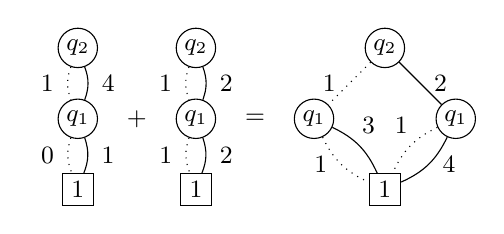
\begin{tikzpicture}[
    scale=0.3,
    every path/.style={>=latex},
    every node/.style={},
    inner sep=0pt,
    minimum size=0.5cm,
    line width=1pt,
    thin,
    font=\small
    ]
    
    % nodes
    
    % nodes
    \node[draw,circle] (a1) at ( 0,-0)     {$q_2$};
    \node[draw,circle] (a2) at (0,-3) {$q_1$};
    
    \node[draw,circle,rectangle,minimum size=0.4cm] (w1) at  (-0,-6) {$1$};
    
    % edges
    \draw[dotted,bend left=-20] (a1) edge  node[left] {$1$} (a2);
    \draw[bend left=20](a1) edge  node[right] {$4$} (a2);
    
    \draw[dotted,bend left=-20] (a2) edge node[left] {$0$} (w1);
    \draw[bend left=20]       (a2) edge  node[right] {$1$} (w1);
    
    
    \node[draw,circle] (a1) at (5,-0)     {$q_2$};
    \node[draw,circle] (a2) at (5,-3) {$q_1$};
    
    \node[draw,circle,rectangle,minimum size=0.4cm] (w1) at ( 5,-6) {$1$};
    
    % edges
    \draw[dotted,bend left=-20] (a1) edge  node[left] {$1$} (a2);
    \draw[bend left=20](a1) edge  node[right] {$2$} (a2);
    
    \draw[dotted,bend left=-20] (a2) edge node[left] {$1$} (w1);
    \draw[bend left=20]       (a2) edge  node[right] {$2$} (w1);
    
    
    \node[draw,circle] (a1p) at ( 13,-0)     {$q_2$};
    \node[draw,circle] (a20) at ( 10,-3) {$q_1$};
    \node[draw,circle] (a21) at ( 16,-3) {$q_1$};
    
    \node[draw,circle,rectangle,minimum size=0.4cm] (w1) at ( 13,-6) {$1$};
    
    % edges
    \draw[dotted] (a1p) edge  node[left] {1} (a20);
    \draw[]     (a1p) edge  node[right] {2} (a21);
    
    \draw[dotted,bend left =-20] (a20) edge  node[left] {1} (w1);
    \draw[      ,bend left = 20]       (a20) edge  node[above right, xshift=-4pt] {3} (w1);
    
    \draw[dotted,bend left =-20] (a21) edge node[above left, xshift=4pt] {1} (w1);
    \draw[      ,bend left = 20]       (a21) edge  node[right] {4} (w1);
    
    
    \node[] (a2) at (2.5,-3) {$+$};
    \node[] (a2) at (7.5,-3) {$=$};
    
\end{tikzpicture}